\newpage
\begin{center}
	\textbf{\large ГЛАВА 5 \\ Разработка ПО}
\end{center}
\refstepcounter{chapter}


% \section*{}
\addcontentsline{toc}{chapter}{ГЛАВА 5}
\section{Общая архитектура}\label{C5_1}

Все взаимодействия комплектующих из пунктов \ref{C4_4_1} - \ref{C4_4_5} происходят путем отправки низкоуровневых комманд из миникомпьютера Orange Pi в соответствующие модули. Команды формируются с помощью программного обеспечения, написанного на высокоуровневом языке Python 3. Данный язык был выбран в связи с наличием динамической типизации, богатой библиотекой для математических вычислений и большой существующей кодовой базой, что позволяет быстро писать прототипы для тестирования. На рисунке \ref{arch} показана структура управления роботом.

\begin{figure}[h!]
	\begin{center}
		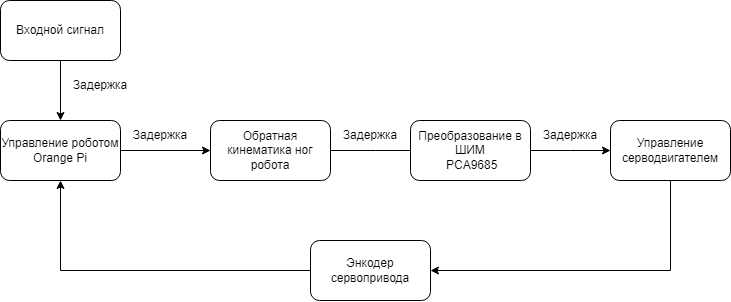
\includegraphics[width=1\textwidth]{arch}
		\caption{Структурная схема управления роботом}
		\label{arch}
	\end{center}
\end{figure}

Система управления роботом интерпретирует входные данные от устройства ввода и преобразует их в траекторию ходьбы для последующего позиционирования тела робота. Блоки обратной кинематической преобразуют координаты ноги в положения сервопривода.

\section{Обратная связь с помощью гироскопа}\label{C5_2}

Главным недостатком такой структуры управления --- недоступность реальных значений углов поворота двигателя, как уже упоминалось в разделе \ref{C4_4_1}, в следствие чего невозможно контролировать ошибку между идеальными и реальными значениями углов вала серводвигателя. Были предложены несколько решений данной проблемы:
\begin{enumerate}
	\item Модификация каждой платы управления сервоприводом;
	\item Подключение гироскопа акселерометра к каждому сервоприводу;
	\item Установка гироскопа акселерометра на корпусе робота.
\end{enumerate}
Первый вариант заключается в демонтаже каждого привода и прямого подключения в выходной сигнал управляющий платы.\newline 
Преимущества:
\begin{itemize}
	\item Получение реальных углов поворота, которые принимают валы двигателей.
	\item Нет необходимости корректировать уравнения кинематики.
	\item Нет необходимости дополнительных вычислений, достаточно учитывать ошибку между реальным и идеальным значением на каждом шаге.
\end{itemize}
Недостатки:
\begin{itemize}
	\item Восемь аналоговых подключений.
	\item OrangePi не поддерживает аналоговые порты.
	\item Требуются дополнительные преобразовательные модули.
	\item Необходимо фильтровать данные.
\end{itemize}
Вывод:
Данное решение, не смотря на его простоту, не является подходящим, так как нет возможности его корректной реализации.
\newline


Второй метод представляет из себя снятие отклонения углов напрямую, преобразуя снятые данные с гироскопа акселерометра. Далее учитывать полученную ошибку на каждом шаге.
\newline
Преимущества:
\begin{itemize}
	\item Получение реальных углов поворота, которые принимают голень и бедро робота.
	\item Нет необходимости корректировать уравнения кинематики.
	\item Нет необходимости лишних вычислений, достаточно учитывать ошибку между реальным и идеальным значением на каждом шаге.
	\item Получаемые данные цифровые. Это позволяет их легко обрабатывать.
\end{itemize}
Недостатки:
\begin{itemize}
	\item Гироскоп акселерометр имеет свойство накапливать ошибку. В данном случае их 8 штук, как следствие, низкая точность.
	\item Восемь цифровых подключений.
	\item Сложность калибровки каждого датчика отдельно.
	\item Требуется дополнительный модуль ``сплиттер'' для подключения более двух гироскопов акселерометров.
	\item Необходимо фильтровать данные.
\end{itemize}
Вывод:
Данное решение не является подходящим, так как необходимы дополнительные модули для работы с гироскопами акселерометрами в количестве более двух штук. Также существенной сложностью является калибровка большого количества датчиков и поддержание необходимой точности вычислений.
\newline


Третий метод заключается в креплении гироскопа акселерометра на корпусе робота и последующего регулирования его отклонений в плоскостях тангажа и крена, тем самым соблюдая условие комфортабельности походки, то есть реализация поступательного, равномерного и прямолинейного движения корпуса.
\newline
Преимущества:
\begin{itemize}
	\item Подключение всего одного датчика.
	\item Малые затраты на реализацию.
	\item Компенсация отклонений корпуса в плоскостях тангажа и рысканья.
	\item Получаемые данные цифровые. Это позволяет их легко обрабатывать.
\end{itemize}
Недостатки:
\begin{itemize}
	\item Необходимо корректировать уравнения кинематики.
	\item Необходимо фильтровать данные
	\item Получаемые данные цифровые. Это позволяет их легко обрабатывать.
\end{itemize}

\noindent В настоящей работе выбран третий вариант, в таком случае структурная схема управления примет вид (см.рисунок \ref{arch_new}).
\newpage
\begin{figure}[h!]
	\begin{center}
		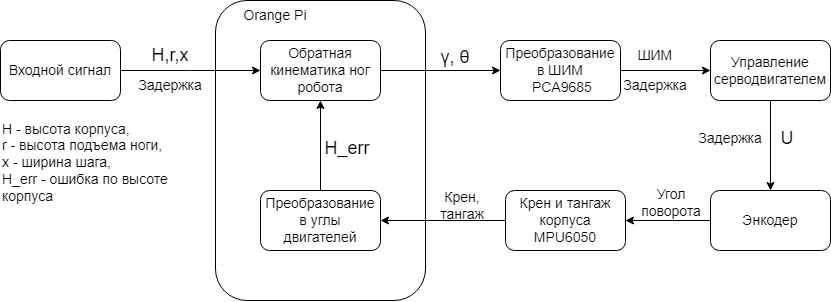
\includegraphics[width=1.2\textwidth,angle=90]{arch_new}
		\caption{Структурная схема управления роботом с обратной связью}
		\label{arch_new}
	\end{center}
\end{figure}
\newpage
\section{Движение робота вперед с обратной связью}\label{C5_3}

Преобразование углов крена и тангажа в углы серводвигателей происходят по алгоритму, описанному ниже:

Для опорный фазы:
\begin{python}
	
    def callculate_step(x_range_step):

		roll_ang,elev_ang = get_pitch_roll() # get data from MPU6050
		elev = np.sin(elev_ang)*body_l//2 # recalculate pitch angle to height
		roll = np.sin(roll_ang)*body_w//2 # recalculate roll angle to height
		y_step=0
		height = drop + elev # include height error (pitch component)
		hip_offset = np.arcsin(elev / body_l) 
		height_slew = np.sqrt(x_range_step**2+(height-y_step)**2)+roll # include height error (roll component) 
		hip_step = 0.5*np.pi - np.arccos(height_slew/(2*self.l1))+np.arctan(x_range_step/(height-y_step)) + hip_offset # conversion to hip servo angle
		knee_step = 2*np.arcsin(height_slew/(2*self.l1)) # conversion to knee servo angle
	
	return np.rad2deg(hip_step), np.rad2deg(knee_step)	
\end{python}

Для свободной фазы аналогично:
\begin{python}
	
    def callculate_skip(x_range_skip,min_delta):
    
		roll_ang,elev_ang = get_pitch_roll() # get data from MPU6050
		elev = np.sin(elev_ang)*body_l//2 # recalculate pitch angle to height
		roll = np.sin(roll_ang)*body_w//2 # recalculate roll angle to height
			
		delta = np.sqrt(self.r**2-min_delta**2)
		y_skip = np.sqrt((self.r**2) - (x_range_skip**2)) - delta
		height = drop + elev # include height error (pitch component)
		hip_offset = np.arcsin(elev / 105)
		height_slew = np.sqrt(x_range_skip**2+(height-y_skip)**2)+roll # include height error (roll component)
		hip_skip = 0.5*np.pi - np.arccos(height_slew/(2*self.l1))+np.arctan(x_range_skip/(height-y_skip)) + hip_offset # conversion to hip servo angle
		knee_skip = 2*np.arcsin(height_slew/(2*self.l1)) # conversion to knee servo angle

	return np.rad2deg(hip_skip),np.rad2deg(knee_skip)
	
\end{python}

Используя данные алгоритмы, получим метрики при движении робота для значений $X_{\text{ш}}$ от $-$50 мм до 50 мм с шагом 1 мм, высотой $h_\text{корп}$ = 150 мм и $r$ = 125 мм. Сравним значения идеальных и реальных углов, полученных с помощью обратной связи.

\begin{figure}[h!]
	\begin{center}
		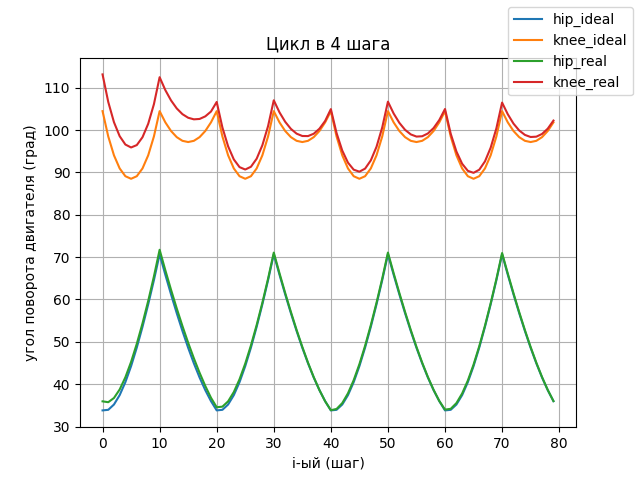
\includegraphics[width=0.9\textwidth]{metrics_servo}
		\caption{Изменение углов двигателей за четыре шага с обратной связью}
		\label{metrics_servo}
	\end{center}
\end{figure}

Исходя из полученного графика можно сделать вывод, что в течение четырех шагов, значения углов на серводвигателях стабилизируются и стремятся к идеальным, что означает работоспособность выбранного метода обратной связи.
\newpage

